% LaTeX support: latex@mdpi.com
%  In case you need support, please attach all files that are necessary for compiling as well as the log file, and specify the details of your LaTeX setup (which operating system and LaTeX version / tools you are using).

% You need to save the "mdpi.cls" and "mdpi.bst" files into the same folder as this template file.

%=================================================================
\documentclass[information,article,submit,moreauthors,pdftex,10pt,a4paper]{Definitions/mdpi}

% If you would like to post an early version of this manuscript as a preprint, you may use preprint as the journal and change 'submit' to 'accept'. The document class line would be, e.g., \documentclass[preprints,article,accept,moreauthors,pdftex,10pt,a4paper]{mdpi}. This is especially recommended for submission to arXiv, where line numbers should be removed before posting. For preprints.org, the editorial staff will make this change immediately prior to posting.

%
%--------------------
% Class Options:
%--------------------
% journal
%----------
% Choose between the following MDPI journals:
% acoustics, actuators, addictions, admsci, aerospace, agriculture, agronomy, algorithms, animals, antibiotics, antibodies, antioxidants, applsci, arts, asi, atmosphere, atoms, axioms, batteries, bdcc, behavsci, beverages, bioengineering, biology, biomedicines, biomimetics, biomolecules, biosensors, brainsci, buildings, carbon, cancers, catalysts, cells, ceramics, challenges, chemengineering, chemosensors, children, cleantechnol, climate, clockssleep, cmd, coatings, colloids, computation, computers, condensedmatter, cosmetics, cryptography, crystals, cybersecurity, data, dentistry, designs, diagnostics, dairy, diseases, diversity, drones, econometrics, economies, education, electrochem, electrochemistry, electronics, energies, entropy, environments, epigenomes, est, fermentation, fibers, fire, fishes, fluids, foods, forecasting, forests, fractalfract, futureinternet, galaxies, games, gastrointestdisord, gels, genealogy, genes, geohazards, geosciences, geriatrics, hazardousmatters, healthcare, heritage, highthroughput, horticulturae, humanities, hydrology, informatics, information, infrastructures, inorganics, insects, instruments, ijerph, ijfs, ijms, ijgi, ijtpp, inventions, j, jcdd, jcm, jcs, jdb, jfb, jfmk, jimaging, jof, jintelligence, jlpea, jmmp, jmse, jpm, jrfm, jsan, land, languages, laws, life, literature, logistics, lubricants, machines, magnetochemistry, make, marinedrugs, materials, mathematics, mca, medsci, medicina, medicines, membranes, metabolites, metals, microarrays, micromachines, microorganisms, minerals, modelling, molbank, molecules, mps, mti, nanomaterials, ncrna, neonatalscreening, neuroglia, nitrogen, nutrients, ohbm, particles, pathogens, pharmaceuticals, pharmaceutics, pharmacy, philosophies, photonics, plants, plasma, polymers, polysaccharides, proceedings, processes, proteomes, publications, quaternary, qubs, reactions, recycling, religions, remotesensing, reports, resources, risks, robotics, safety, sci, scipharm, sensors, separations, sexes, sinusitis, smartcities, socsci, societies, soilsystems, sports, standards, stats, surfaces, surgeries, sustainability, symmetry, systems, technologies, toxics, toxins, tropicalmed, universe, urbansci, vaccines, vehicles, vetsci, vibration, viruses, vision, water, wem, wevj
%---------
% article
%---------
% The default type of manuscript is article, but can be replaced by:
% abstract, addendum, article, benchmark, book, bookreview, briefreport, casereport, changes, comment, commentary, communication, conceptpaper, correction, conferenceproceedings, conferencereport, expressionofconcern, extendedabstract, meetingreport, creative, datadescriptor, discussion, editorial, essay, erratum, hypothesis, interestingimages, letter, meetingreport, newbookreceived, opinion, obituary, projectreport, reply, reprint, retraction, review, perspective, protocol, shortnote, supfile, technicalnote, viewpoint
% supfile = supplementary materials
% protocol: If you are preparing a "Protocol" paper, please refer to http://www.mdpi.com/journal/mps/instructions for details on its expected structure and content.
%----------
% submit
%----------
% The class option "submit" will be changed to "accept" by the Editorial Office when the paper is accepted. This will only make changes to the frontpage (e.g., the logo of the journal will get visible), the headings, and the copyright information. Also, line numbering will be removed. Journal info and pagination for accepted papers will also be assigned by the Editorial Office.
%------------------
% moreauthors
%------------------
% If there is only one author the class option oneauthor should be used. Otherwise use the class option moreauthors.
%---------
% pdftex
%---------
% The option pdftex is for use with pdfLaTeX. If eps figures are used, remove the option pdftex and use LaTeX and dvi2pdf.

%=================================================================
\firstpage{1}
\makeatletter
\setcounter{page}{\@firstpage}
\makeatother
\pubvolume{xx}
\issuenum{1}
\articlenumber{5}
\pubyear{2019}
\copyrightyear{2019}
%\externaleditor{Academic Editor: name}
\history{Received: date; Accepted: date; Published: date}
%\updates{yes} % If there is an update available, un-comment this line

%% MDPI internal command: uncomment if new journal that already uses continuous page numbers
%\continuouspages{yes}

%------------------------------------------------------------------
% The following line should be uncommented if the LaTeX file is uploaded to arXiv.org
%\pdfoutput=1

%=================================================================
% Add packages and commands here. The following packages are loaded in our class file: fontenc, calc, indentfirst, fancyhdr, [demo]graphicx, lastpage, ifthen, lineno, float, amsmath, setspace, enumitem, mathpazo, booktabs, titlesec, etoolbox, amsthm, hyphenat, natbib, hyperref, footmisc, geometry, caption, url, mdframed, tabto, soul, multirow, microtype, tikz

\usepackage{caption}
\usepackage{subcaption}
\usepackage{todonotes}

%=================================================================
%% Please use the following mathematics environments: Theorem, Lemma, Corollary, Proposition, Characterization, Property, Problem, Example, ExamplesandDefinitions, Hypothesis, Remark, Definition
%% For proofs, please use the proof environment (the amsthm package is loaded by the MDPI class).

%=================================================================
% Full title of the paper (Capitalized)
\Title{Large Scale Linguistic Processing of Tweets to Understand Social Interactions among Speakers of Less Resourced Languages: The Basque Case}

% Authors, for the paper (add full first names)
\Author{Joseba Fernandez de Landa, Rodrigo Agerri* and I\~naki Alegria}

% Authors, for metadata in PDF
\AuthorNames{Joseba Fernandez de Landa, Rodrigo Agerri, I\~naki Alegria}

% Affiliations / Addresses (Add [1] after \address if there is only one affiliation.)
\address[1]{%
IXA NLP Group, University of the Basque Country UPV/EHU\\
%$^{2}$ \quad Affiliation 2; e-mail@e-mail.co
}

% Contact information of the corresponding author
\corres{Correspondence: joseba.fdl@gmail.com, rodrigo.agerri@ehu.eus}

% Current address and/or shared authorship
%\firstnote{Current address: Affiliation 3}
%\secondnote{These authors contributed equally to this work.}
% The commands \thirdnote{} till \eighthnote{} are available for further notes

%\simplesumm{} % Simple summary

% Abstract (Do not insert blank lines, i.e. \\)
\abstract{Social networks like Twitter are taking more and more importance nowadays, creating new ways of communication. They are also a useful tools for social and linguistic research, because there is a lot of public data available based on social interaction using such networks. The availability of this data is particularly important for less resourced languages, allowing to apply current Natural Language Processing techniques to large amounts of unstructured data in order to analyze both the linguistic and social behaviour of users based on the text they generate. In this work, we aim to study the linguistic and social aspects of young and adult people’s behaviour based on their tweets' contents and the social relations that arise from them. With this objective in mind, we have gathered over 10 million tweets written in Basque from more than 8000 users. First, we extracted and analyzed the crawled data to find the most popular topics. Then we classified each user in terms of its life stage (young/adult) by establishing whether the writing style of the tweets is formal or informal. Several classification and topic modelling methods, both supervised and unsupervised, have been applied, offering each of them different insights with respect to the feasibility of the task with the available data. Second, we established the relations that emerge between the users based on their retweets, characterizing also the various communities that emerge from the analysis of the data. We conclude that social research can be done using computational techniques such as Natural Language Processing, giving the opportunity both to segment communities based on demographic characteristics and to discover how they interact or relate to them, using large amounts of unstructured data.}

% Keywords
\keyword{Social Informatics; Social Networks; Topic Modelling; Relations; Less Resourced Languages; Text Classification; Information Extraction; Natural Language Processing}

% The fields PACS, MSC, and JEL may be left empty or commented out if not applicable
%\PACS{J0101}
%\MSC{}
%\JEL{}

%%%%%%%%%%%%%%%%%%%%%%%%%%%%%%%%%%%%%%%%%%
% Only for the journal Data:
%\dataset{DOI number or link to the deposited data set in cases where the data set is published or set to be published separately. If the data set is submitted and will be published as a supplement to this paper in the journal Data, this field will be filled by the editors of the journal. In this case, please make sure to submit the data set as a supplement when entering your manuscript into our manuscript editorial system.}

%\datasetlicense{license under which the data set is made available (CC0, CC-BY, CC-BY-SA, CC-BY-NC, etc.)}

%%%%%%%%%%%%%%%%%%%%%%%%%%%%%%%%%%%%%%%%%%
\begin{document}

%The order of the section titles is: Introduction, Materials and Methods, Results, Discussion, Conclusions for these journals: aerospace,algorithms,antibodies,antioxidants,atmosphere,axioms,biomedicines,carbon,crystals,designs,diagnostics,environments,fermentation,fluids,forests,fractalfract,informatics,information,inventions,jfmk,jrfm,lubricants,neonatalscreening,neuroglia,particles,pharmaceutics,polymers,processes,technologies,viruses,vision


\section{Introduction}\label{sec:introduction}


In the last few years Twitter has become one of the most used social networks, creating new ways of consuming information but also of communicating and creating both leisure- and work-related relationships in a explicit manner but also implicitly, via the information we shared with our followers via retweets. Furthermore, nowadays Twitter has become a source of spontaneously generated textual data for many human languages, including less resource languages such as Basque. Thus this data is becoming more and more useful to do social and computational linguistic research \cite{nguyen2016computational,rosenthal2017semeval,baldwin2015shared} both to complement traditional methods of sociological research and to provide with massive amounts of textual data to apply modern techniques of Natural Language Processing (NLP) based on machine and deep learning, for tasks such as automatic analysis of opinions (Opinion Mining or Sentiment Analysis) \cite{rosenthal2017semeval,S16-1003}, Named Entity Recognition and Lexical Normalization \cite{baldwin2015shared}, fake news and rumour detection \cite{derczynski2017semeval}, among others.

In this paper we present a multidisciplinary work that aims to contribute novel insights in social research by using and investigating techniques from Natural Language Processing based on the general background proposed by Bauman and his \emph{liquid society} \cite{bauman2013liquid}. Thus, the objective of this work is to provide a detailed social and demographic-based view of the most important topics and relationships that are formed between Basque Twitter users classified by life stage (young and adult). By ``Basque Twitter users'' we refer to those users that are geolocalized in the area of the Basque Country (cultural) and that write at least the 20\% of their tweets using the Basque language. This analysis will be entirely based on automatically collected tweets from Basque users.

More specifically, the work presented in this paper will consist of the following main steps. First, we will identify the relevant Basque Twitter users. Second, a large corpus of tweets will be extracted using the identified users' timelines. Third, we will classify users in terms of life stage (adult/young) by classifying the writing style of the tweets in their timelines as \emph{formal} or \emph{informal}. This is due to the fact that we do not have metadata information about the users' age, which means that we have to somehow try to infer the life stage based on features about writing style. Five different classification methods will be investigated, including the use of machine learning techniques based on both feature-based and neural network architectures. We will use the classifier with the best results in order to label the large corpus of Basque tweets by their writing style thereby classifying their users in terms of \emph{young} or \emph{adult}. In the final step, this classification will be used to investigate the most relevant topics among users of Twitter writing in Basque as well as for researching the social relations that emerge between each user type (young or adult). The final result will be a comprehensive sociological picture (automatically obtained) of the most important aspects within the community of Basque users of Twitter.

The main contributions of this work are the following. First, we collect and publish a corpus of 6M tweets written in Basque and a manually annotated gold-standard of 1000 tweets in terms of the writing style, namely, \emph{formal} or \emph{informal}. Both corpora are made available to facilitate both NLP and social research in Basque\footnote{\url{https://github.com/ixa-ehu/heldugazte-corpus}}, a less resource highly-inflected language. Second, we investigate the classification of Basque tweets as \emph{formal} or \emph{informal} using 5 different approaches including novel NLP techniques based on word embeddings, contextual character embeddings and neural networks. We believe that our work is the most comprehensive experimentation for the detection of users' age both in terms of number of users and NLP techniques used. Third, the models of the best system will be made publicly available to facilitate their use and reproducibility of results\footnote{\url{https://github.com/ixa-ehu/ixa-pipe-doc}}. An interesting insight from this part is the fact that, contrary to common views, the neural approach \cite{akbik2018contextual} obtains very competitive results despite being trained on a very small dataset. We believe that is due mostly to the combination of character-based contextual embeddings with static word embeddings. Fourth, we perform the largest investigation of social relationships in terms of age stages for Basque communities based on an automatically classified corpus of almost 8K users and 6M tweets. Finally, we believe that this work shows how to make it possible to do meaningful and large scale social and NLP research for less resource languages using texts from social media. In our view, this work is just the beginning.

\section{Related Work}\label{sec:background}

Analyzing demographic characteristics in social media is receiving increasing attention in the area of Social Media Mining \cite{nguyen2016computational,morgan2017predicting}. The popularity of Twitter has in fact benefited such approaches as it is possible now to mine spontaneous contributions and opinions of users about any kind of topic in many languages, including less resource languages. At the same time, by taking into account the relations created between retweets will allow us to analyze and try to understand the type of relations and user communities that are being created within the social network. Both social and linguistic aspects are important for our work as we will try to perform social and demographic analysis via large scale linguistic processing on written texts extracted from a social network such as Twitter. The main techniques used here are those related to topic modelling, the study of social relationships and text processing or Natural Language Processing (NLP).

With respect to topic modelling, many different approaches have tried to extract common information contained in large amounts of tweets scattered through the network, such as topic extraction with respect to an event and their related tweets \cite{hu2012lda}, real-time classification of twitter trends \cite{zubiaga2015real} or to compare the content of Twitter with traditional news media \cite{zhao2011comparing}. Applying topic modelling to tweets, like for other tasks, requires some pre-processing to make the task appropriate for such short texts or documents \cite{hong2010empirical}.

In relation to the study of the social relationships that are generated within the network, closer to use are those studies that have aimed to identify communities of users based on their retweets. Among these, one can find studies about political polarization \cite{conover2011political}, political affiliation detection \cite{pennacchiotti2011democrats} or even studies about identifying communities in movements for independence \cite{zubiaga2017stance}. In these studies, based on the retweets made by the user, it is shown that there identification of communities or groups is quite feasible. In our work we will use similar methodologies to the ones mentioned here with the objective of uncovering latent communities formed within Basque users of Twitter.

The use of Twitter is very popular in the area of Natural Language Processing (NLP), where tweets are used for many tasks such as mining opinions about specific products or topics \cite{rosenthal2017semeval,villena2013tass}, analyzing stance detection and fake news \cite{S16-1003,zubiaga2017stance} or in more low level NLP tasks such as POS tagging \cite{ritter_named_2011}, Named Entity Recognition \cite{baldwin2015shared}, normalization \cite{alegria2015tweetnorm} and language identification \cite{zubiaga2016tweetlid}, among many others. Previous NLP work is relevant to us as we will work with tweets to perform text classification with the aim of labelling tweets according to their writing style (conventional-informal or formal), although we will be working on our specifically created gold dataset of Basque tweets. The results of this work will allow us to classify Twitter users by their life stage (young or adult) which in turn would allow us to analyze their demographic characteristics with respect to the most important topics and with respect to the type of social relations that get created.

Of particular interest to us is the body of work performed with the objective of age or life stage detection for Twitter users. Table \ref{tab:arte ezaug} lists the most relevant work on this task. Most of them create their own datasets with manually annotated data to learn life stages or age ranges. As it can be seen the number of users varies from 300 to 3000. It is also important to mention that the best performing systems are those that use at most two  \cite{rao2010classifying,al2012homophily} or three \cite{nguyen2013old,morgan2017predicting} labels denoting the life stages of interest for the classification task.

\begin{table}[H]
  \centering
  \begin{tabular}{llcr}\hline
    Reference & Corpus size \# users & \# labels & Language \\ \hline \hline
    Rao et al. (2010) & 1000 & 2 & en \\
    Al Zamal et al. (2012) & 400 & 2 & en \\
    Marquart et al. (2014) & 306 & 5 & es \\
    Nguyen et al. (2013) & 3110 & 3 & nl \\
    Morgan-Lopez et al. (2017) & 3184 & 3 & en \\ \hline
  \end{tabular}
  \caption{Most relevant systems for age detection in Twitter.}
  \label{tab:arte ezaug}
\end{table}

For the task of age detection, most of previous works use both the text and the metadata provided by the Twitter API, most importantly the age of each user in order to guide the supervised learning methods. Previous work is based on Logistic Regression \cite{nguyen2013old,morgan2017predicting} and Support Vector Machines \cite{rao2010classifying,al2012homophily,marquardt2014age}. Best results in this area obtained 86.32 word accuracy \cite{nguyen2013old} for three age or life stages, although others scored well below that, most of them ranging around 74-80 word accuracy. These comparatively lower scores makes it more difficult to perform meaningful social and demographic research using such automatic classifiers. Therefore, an important contribution of this work will be to strive in providing good performing and classifiers for Basque tweets but also with the aim of the models to be robust and general enough to be applicable for different text classification tasks across different languages.


% #########################################################
% ################     DATA EXTRACTION     ################
% #########################################################
% Euskal txiolarietaz gain ere, modu orokorrago batean azaldu ataza (abstrakzio malia altuagoa) -->> hiztun gutxituen komunitateari buruzko analisia.

\section{Extracting a Large Corpus of Tweets from Basque Users}\label{sec:data-extraction}

As we have already commented in the introduction, Twitter allows to obtain relatively large datasets to work with even for less resourced languages. Before starting to collect the data, we defined the community of users that will be the subject (or, in other words, the universe) of our study. In our case the choice was quite simple, namely, we wanted to use tweets from every Twitter user that publishes tweets in Basque. The task of identifying such users was facilitated thanks to UMAP, a platform that monitors every tweet written in Basque. More specifically, UMAP includes a list of users who publish at least 20\% of their tweets in Basque. We used such source to obtain a list of 8189 users.

The Twitter API was used via the tweepy package, choosing the \textit{timeline extraction} mode to gather the last 3,200 available tweets of each of the 8189 users in our sample. The data collection was performed between May 30th and 31st of 2018, gathering, after some errors, more than 10 million (multilingual) tweets from 7980 users. We call this data the \emph{Large Corpus}. Next, we classify the tweets by language using the metadata provided by the Twitter API, identifying those that are written in Basque. The result is a dataset of around 6M tweets that we refer to as the \emph{Heldugazte Corpus}, which we split in personal tweets and retweets. The main statistics of the Heldugazte corpus are provided by Table \ref{tab:useful-data}\footnote{The corpus is publicly available at \url{https://github.com/ixa-ehu/heldugazte-corpus}.}.

\begin{table}[H]
  \centering
  \begin{tabular}{lll} \hline
     & Personal tweets in Basque & Retweets in Basque \\ \hline \hline
    Tweets & 3,171,785 & 2,891,136 \\
    Terms & 1,434,050 & 813,833 \\
    Tokens & 37,350,268 & 39,329,204 \\ \hline
  \end{tabular}
  \caption{Characteristics of the Heldugazte corpus.}
  \label{tab:useful-data}
\end{table}

\section{Classifying Users by Age Stage}\label{sec:class-young-users}

In this section we present our work to classify Basque Twitter users as young or adult by analyzing their tweets' writing style. As we have seen in Section \ref{sec:background}, previous work includes automatic approaches to characterize users in the context of social networks and media, the most common being those related with genre and age \citep{cesare2017detection}. Our objective of developing a classifier to characterizing Basque Twitter users according to two stages of life (young/adult) is therefore placed within that research line.

Furthermore, Section \ref{sec:background} also shows that most of previous work addresses the problem of classifying age stages using supervised machine learning techniques. This implies that some training data must be annotated according to the age or age stage of each user. Moreover state of the art  results indicate that classifying by age stages allows to obtain better results than when the problem is formulated in terms of age ranges \citep{nguyen2013old}. This seems to be due to the fact that shared experiences are easier to relate along time by using age stages rather than age ranges \citep{nguyen2016computational,eckert2017age}. Therefore, in this work we decided to focus on classifying users in terms of two general age stages, namely, young and adult.

However, this decision encountered an early methodological problem. In order to annotate tweets written in Basque according to the age stages of their authors it is obviously necessary to have available some data providing such information. Unfortunately, for the large majority of users from which we mined tweets this information is not available. Thus, our decision to overcome this problem consisted of focusing on the information available on the tweets themselves by taking into account writing style features. After all, most of the previous work widely uses writing style based features in order to classify users in terms of age stages \citep{rao2010classifying,al2012homophily,nguyen2013old,morgan2017predicting}.

It has been suggested that adults tend to use more conventional language \cite{nguyen2013old} whereas for young people it is more common to display repetitions and out of dictionary words \citep{rao2010classifying,rosenthal2011age,morgan2017predicting}. Generalizing on this idea we will assume that writing style changes according to the age of the twitter user. In other words, we will consider that \emph{adult writing style} is more formal whereas young people's style can be seen as more informal. Therefore, we will be classifying users as young/adult by classifying their tweets in terms of formal or informal language.

\subsection{Experimental Framework}\label{sec:exper-fram}

Following the setting established above, we will address the problem of classifying each tweet as \emph{formal} or \emph{informal} by means of several approaches. First, we will apply a statistical method based on perplexity \cite{gamallo2017language}. Second, we will experiment with several supervised methodologies: (i) a baseline method using sparse, \emph{one-hot} word representations \cite{pedregosa2011scikit}; (ii) a feature-based method using word representations as continuous word vectors, namely, word embeddings, on top of the baseline developed in (i) \cite{mikolov2013distributed,pennington-etal-2014-glove,mikolov-etal-2018-advances}; (iii) an off-the-shelf system which uses clustering features for representing the documents \cite{agerri2016robust,agerri2019language} and (iv), a deep learning approach leveraging character contextual word embeddings and a neural network architecture \cite{akbik2018contextual}.

We will develop a classifier with each of the methods listed above and evaluate it on a held-out, gold-standard dataset manually annotated at tweet level for the categories of \emph{formal} and \emph{informal}. The method that obtains the best results in the experiments will be then used to annotate the 6 million tweets obtained thereby classifying their authors as \emph{young} or \emph{adult}. In this sense, users will be classified according to the writing style of the tweets in their timelines.

In the rest of this section we will describe the process of manual annotation of the training and evaluation data. After that, we describe the configuration settings of each of the systems used or implemented for the experiments.

\subsubsection{The Heldugazte Gold Standard Corpus}\label{sec:gold-standard-data}

In order to focus on learning to classify tweets according to writing style, we decided to clean the tweets keeping only those words that contained alphanumeric characters. Thus, we removed emoticons, hashtags, users' names (@) and URL links. Furthermore, we only considered those tweets that contained more than 4 tokens. We then randomly selected 1000 tweets sent from personal accounts from the 6 million tweet dataset collected as described in Section \ref{sec:data-extraction}. One annotator manually labeled every tweet as \emph{formal} or \emph{informal}.

\begin{table}[H]
  \centering
  \begin{tabular}{lr} \hline \hline
    Total number of tweets & 1.000 \\
    Formal & 492 \\
    Informal & 508 \\
    Tokens in shortest tweet & 5 \\
    Tokens in longest tweet & 34 \\
    Token avg. & 9.66 \\ \hline
  \end{tabular}
  \caption{The Heldugazte gold standard corpus.}
  \label{tab:gold-corpus}
\end{table}

To manually label the tweets, a qualitative methodology was followed: all those tweets that contained out of vocabulary words or colloquial expressions were classified as informal. This methodology has been motivated by previous work on classifying formal and colloquial tweets \cite{gonzalez2015analysis}. Table \ref{tab:gold-corpus} shows the main features of our manually annotated dataset. For the experiments described in the next four subsections, we split the gold standard corpus in three sets, leaving 65\% for training and \%35 for testing\footnote{The Heldugazte gold-standard corpus is publicly available at \url{https://github.com/ixa-ehu/heldugazte-corpus}.}. In the following we present two examples of the type of tweets we classify in this work. In both cases it can be seen the differences in writing style. Thus, in the informal tweets appear dialectal and/or slang forms (ein, examin, bau, det), whereas the formal tweet displays quite a standard Basque grammar.

\begin{itemize}
\item[(1)] \textbf{Informal tweet}: ``inoizz ezdet ein mateko examin bau au baino okerro''\footnote{Informal: This is worst exam I have ever done.}
\item[(2)] \textbf{Formal tweet}: ``killian jornet fenomenoa da zegamaaizkorri irabazi du beste behin non dago mendizale gazte honen muga''.\footnote{Formal: Killian Jornet is a phenomenon he won the Zegama-Aizkorri again. Where is this mountaineer's limit?}
\end{itemize}

\subsubsection{Perplexity-based Distance}\label{sec:unsup-appr-text}

Perplexity is a widely-used evaluation metric for language models built with n-grams extracted from text corpora \cite{chen1999empirical}. Furthermore, it has been used for specific tasks, namely, to classify between formal and colloquial tweets \cite{gonzalez2015analysis} or for language identification between similar languages \cite{gamallo2017language}. Both works inspire our approach to classifying tweets as formal or informal using perplexity. The former showed that perplexity could be useful to indirectly detect out-of-vocabulary words in tweets \cite{gonzalez2015analysis}. More importantly for us, the latter formally proposed the concept of \emph{perplexity-based distance} between two languages.

A perplexity-based distance between two languages is established by ``comparing the n-grams of a text in one language with the n-gram language model trained for the other language. Then, the perplexity of a test text T in language L2, given the language model LM of language L1, can be used to define the distance, between L1 and L2'' \cite{gamallo2017language}. According to this definition, low perplexity indicates close proximity between languages L2 and L1.

In order to classify tweets as \emph{formal} or \emph{informal}, we will calculate the perplexity-based distance between a tweet with respect to a character-based 7-gram language model. If the perplexity-based distance between each tweet and the character-based n-gram language model is low, then we will classify it as \emph{formal} and \emph{vice versa}. Of course, for this approach to work we need to establish a threshold so that if the perplexity-based distance is lower than the threshold the tweet is labeled as \emph{formal} and if higher, as \emph{informal}.

Our method to calculate such threshold proceeds in the following manner. First, we build a 7-gram character-based language model using the data from a corpus composed of texts from the Basque  Egunkaria and Berria newspapers. Second, we take the tweets in the training set (65\% of the dataset) and classify each of them according to the perplexity-based distance with respect to the language model. We tried every value in the [0,10] range
with an increment of 0.1 as threshold. Third, we computed precision, recall and accuracy comparing the prediction of the threshold according to the perplexity value with respect to the gold-standard labels in the training data. Finally, the threshold chosen will be the value in which all the three metrics converge. As shown by Figure \ref{fig:threshold}, we found out that the best threshold value was around 4.4. We will use this value in order to evaluate this approach in Section \ref{sec:experimental-results}.

\begin{figure}[H]
 \centering
 \begin{subfigure}[b]{0.49\linewidth}
   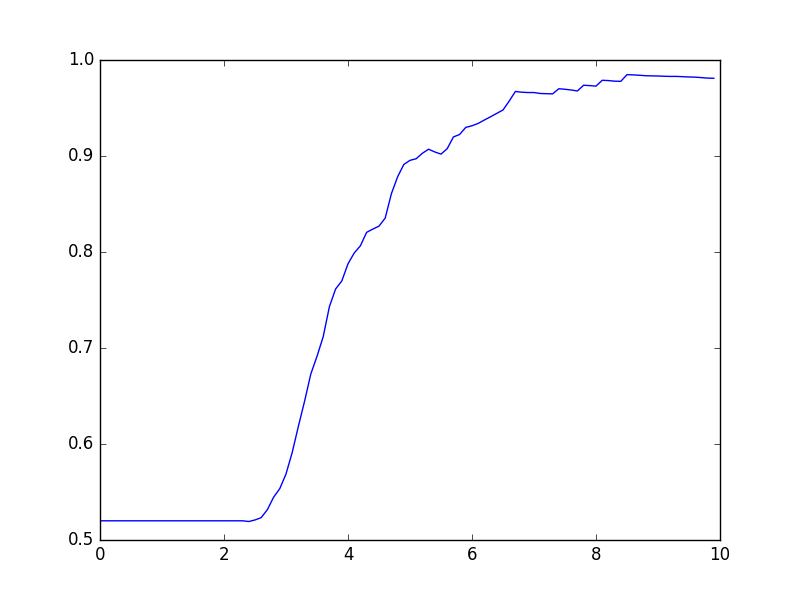
\includegraphics[width=\linewidth]{precision}
 \end{subfigure}
 \begin{subfigure}[b]{0.49\linewidth}
   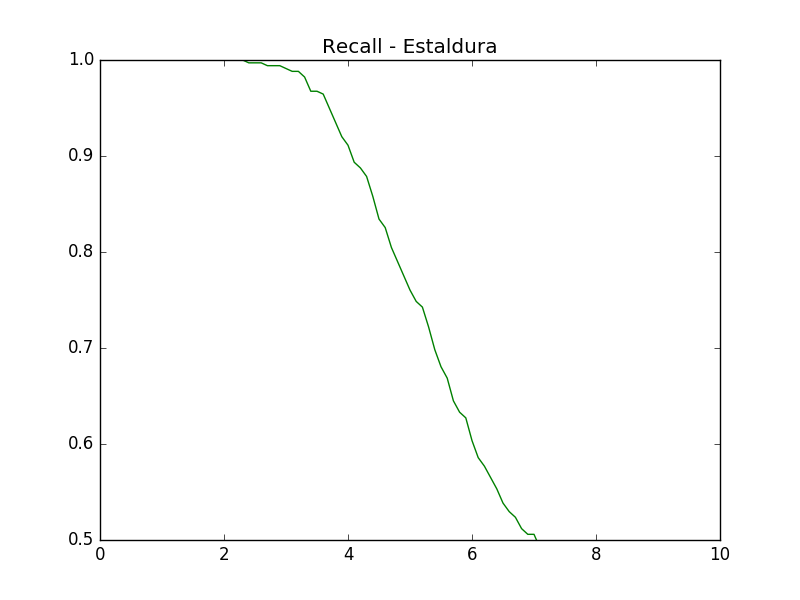
\includegraphics[width=\linewidth]{recall}
 \end{subfigure}
 \begin{subfigure}[b]{0.49\linewidth}
   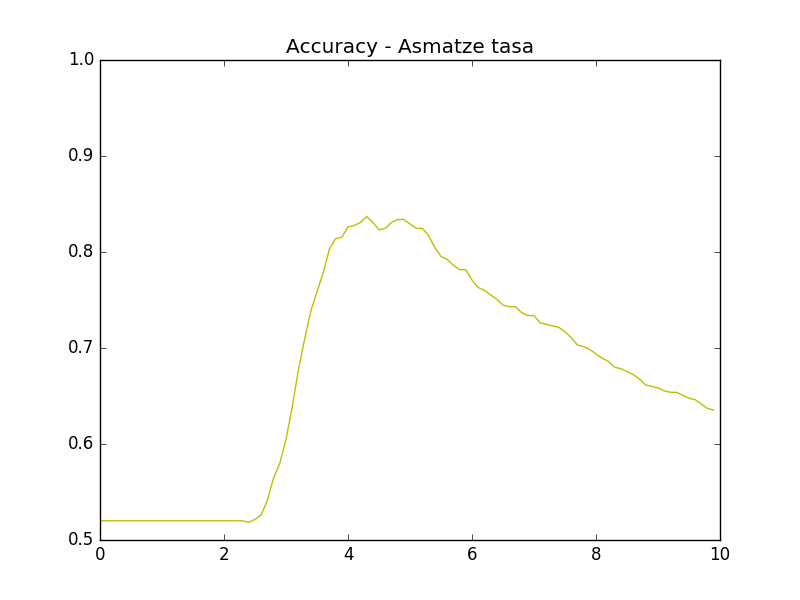
\includegraphics[width=\linewidth]{accuracy}
 \end{subfigure}
 \begin{subfigure}[b]{0.49\linewidth}
   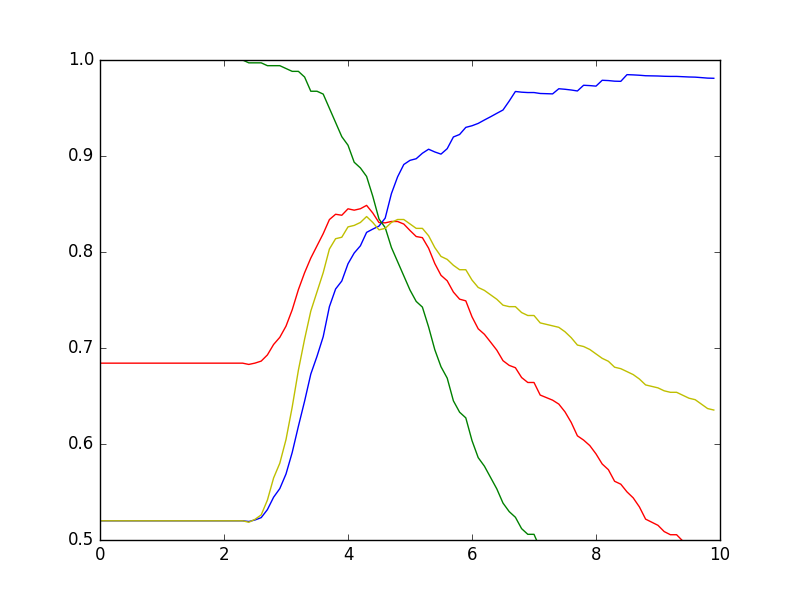
\includegraphics[width=\linewidth]{denaperp}
 \end{subfigure}
   \caption{Finding the optimal threshold value (down, right) on the training data using Precision (top left), Recall (top right) and Accuracy (left, down) curves.}\label{fig:threshold}
\end{figure}

% \begin{figure}[H]
%   \centering
%     \subfloat[Precision.]{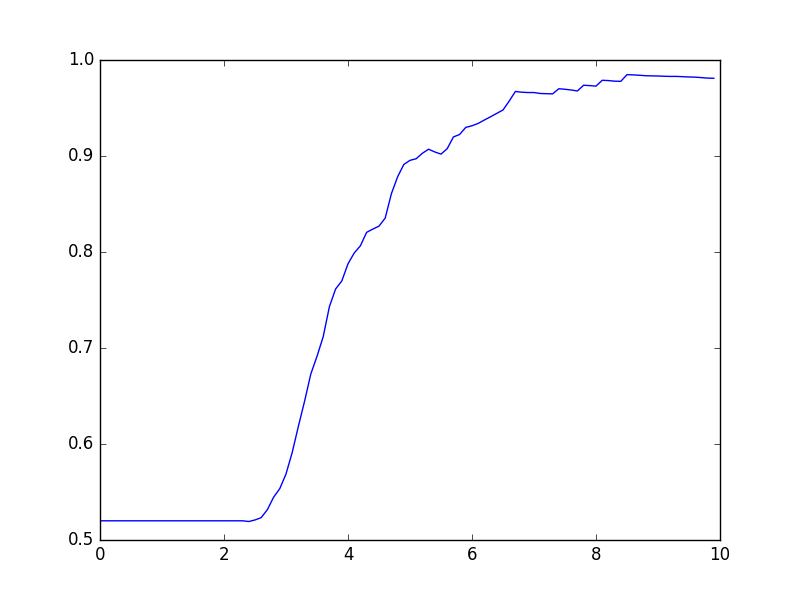
\includegraphics[width = .5\linewidth]{precision}}
%     \subfloat[Recall.]{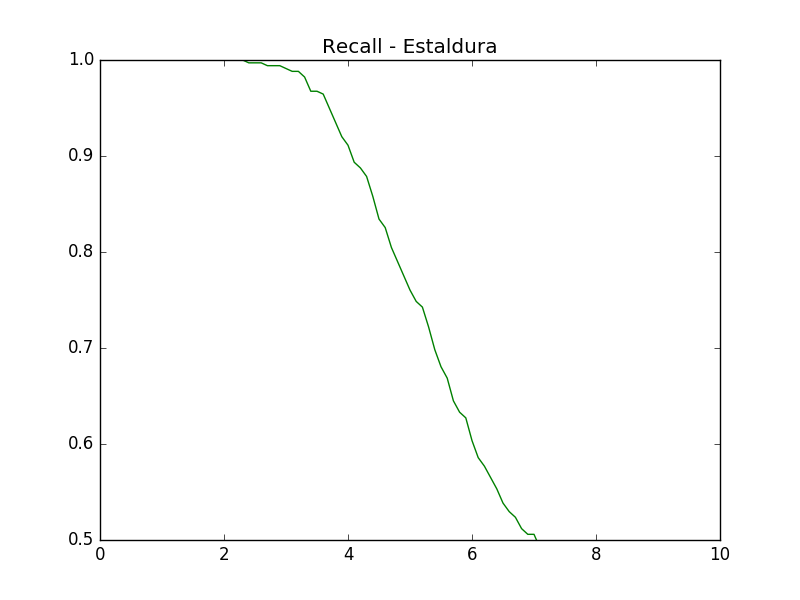
\includegraphics[width = .5\linewidth]{recall}}\\
%     \subfloat[Accuracy.]{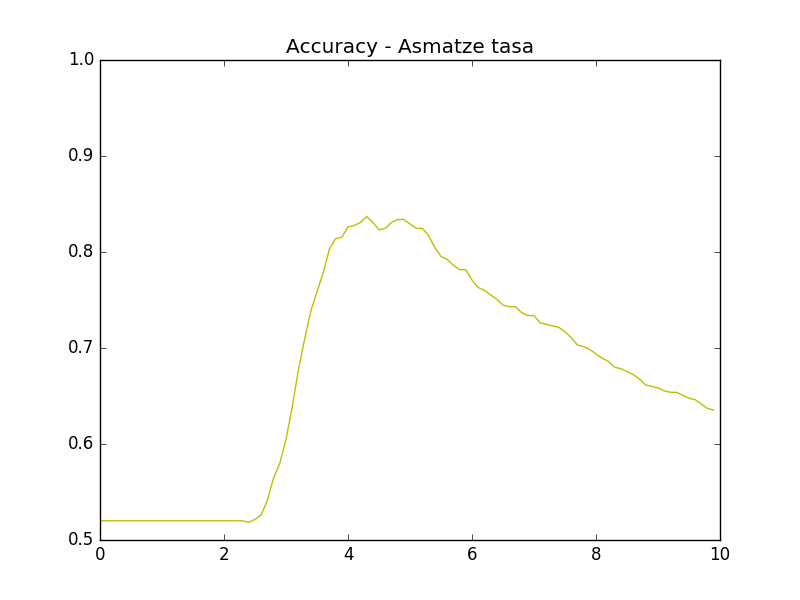
\includegraphics[width = .5\linewidth]{accuracy}}
%     \subfloat[Optimal threshold value on the training data.]{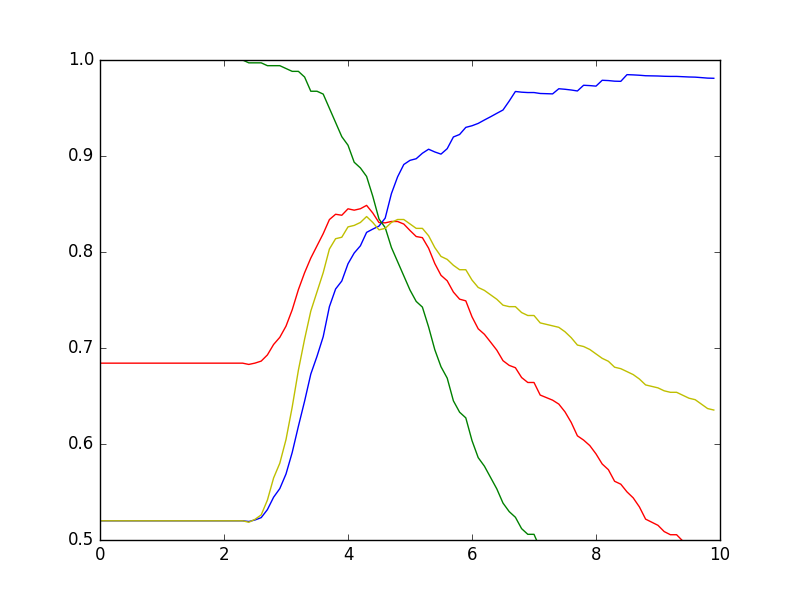
\includegraphics[width = .5\linewidth]{denaperp}}
% \caption{Obtaining the optimal threshold value on the training data.}\label{fig:threshold}
% \end{figure}

Table \ref{tab:perplexitytrain} displays the results of classifying the tweets in the training data using perplexity-based distance using the value 4.4 as threshold. The obtained overall accuracy using 4.4 as threshold was 0.831.

\begin{table}[H]
  \centering
  \begin{tabular}{lcccc} \hline
    Label & Error & Precision & Recall & F1 \\ \hline \hline
    Informal & 48 & 0.824  & 0.858  & 0.841 \\
    Formal & 62 & 0.839 & 0.801 & 0.820 \\ \hline
  \end{tabular}
  \caption{Results of the perplexity-based approach on the training set.}
  \label{tab:perplexitytrain}
\end{table}

\subsubsection{Supervised Baseline}\label{sec:sparse-word-repr}

The first baseline applying supervised machine learning will be done to test various learning algorithms using the gold standard dataset described in Section \ref{sec:gold-standard-data}. More specifically, we will be simply applying a bag of words representation which represents each document (tweet) according to the word frequencies in each document. The result is a very sparse word representation where the dimension of the vector representing each word is equal to the number of words in the corpus. In this setting, we apply six of the most common machine learning algorithms with default parameters using the scikit-learn library \cite{pedregosa2011scikit}. Table \ref{tab:acc-ml} reports their performance by means of 5-fold cross validation on the training data.

\begin{table}[H]
  \centering
  \begin{tabular}{lr} \hline
    Machine Learning Classifier (BoW) & Accuracy \\ \hline \hline
    5-NN (k-NN) &  0.614 \\
    Decision Tree &  0.677 \\
    Random Forest &  0.707 \\
    Naive Bayes & 0.765 \\
    Logistic Regression & 0.775 \\
    \textbf{SVM} & \textbf{0.777} \\ \hline
  \end{tabular}
  \caption{Bag of words results via 5-fold cross-validation on the training set.}
  \label{tab:acc-ml}
\end{table}

As it can be seen, the best performing algorithms in this baseline setting are Logistic Regression and SVM. This is not surprising given the ability of SVM to perform well with very few labeled data. Next, we decided to experiment with a less-sparse representation of the tweets by means of pre-trained word embeddings and the SVM classifier.

\subsubsection{Pre-trained Word Embeddings}\label{sec:pre-trained-word}

Distributed word representations or word embeddings are widely used nowadays in Natural Language Processing. Several techniques have been proposed in order to obtain word embeddings, most of them based on the hypothesis that the meaning of a word is defined by the context in which it appears \cite{mikolov2013distributed,pennington-etal-2014-glove}. Thus, obtaining word embeddings usually requires large quantities of good quality training data which makes it difficult when experimenting with less-resourced languages such as Basque. However, FastText provides pre-trained models for many languages, including Basque \cite{mikolov-etal-2018-advances} by using the common crawl data\footnote{\url{http://commoncrawl.org}}. The Basque model they distribute is trained on both Common Crawl and Wikipedia using CBOW with position-weights, in 300 dimension, with character n-grams of length 5, a window of size 5 and 10 negatives\footnote{\url{https://fasttext.cc}}.

For this experiment, we map the words in the corpus to their real vector representation in the FastText model and average all the vectors with respect to the vocabulary. We optimize the C hyperparameter using accuracy and evaluate by 5-fold cross-validation on the training data. Table \ref{tab:svmf1} reports the detailed results of the 5-fold cross-validation using C$=1.1$ as hyperparameter.

\begin{table}[H]
  \centering
  \begin{tabular}{lcccc}
    \hline
    Label & Error & Precision & Recall & F1 \\ \hline \hline
    Informal & &  &   &  \\
    Formal &  &  &  &  \\ \hline
  \end{tabular}
  \caption{SVM (rbf and FastText embeddings) results via 5-fold cross-validation on the training set.}
  \label{tab:svmf1}
\end{table}

\subsubsection{IXA pipes}\label{sec:ixa}

The document classification system included in the IXA pipes tools, \emph{ixa-pipe-doc}, aims to establish a simple and shallow feature set, avoiding any linguistic motivated features, with the objective of removing any reliance on costly extra gold annotations and/or cascading errors if automatic annotations are used. The underlying motivation is to obtain robust models to facilitate the development of document classification systems for several languages, datasets and domains while obtaining state of the art results.

\emph{ixa-pipe-doc}, as a component of IXA pipes, includes a simple method to combine various types of clustering features induced over different data sources or corpora. This method has already obtained state of the art results in several tasks such as newswire Named Entity Recognition \cite{agerri2016robust} and Opinion Target Extraction \cite{agerri2019language}, both in out-of-domain and in-domain evaluations and for several languages, including Basque.

The system consists of: (i) Local, shallow features based mostly on orthographic, word shape and n-gram features plus their context; (ii) three types of simple clustering features, based on unigram matching; (iii) publicly available gazetteers, such as sentiment lexicons. Specifically, \emph{ixa-pipe-doc} implements, on top of the local features, a combination of word representation features: (i) Brown \cite{brown1992class} clusters, taking the 4th, 8th, 12th and 20th node in the path; (ii) Clark \cite{clark2003combining} clusters and, (iii) Word2vec \cite{mikolov2013distributed} clusters, based on K-means applied over the extracted word vectors using the skip-gram algorithm. The implementation of the clustering features looks for the cluster class of the incoming token in one or more of the clustering lexicons induced following the three methods listed above. If found, then we add the class as feature. The Brown clusters only apply to the token related features, which are duplicated\footnote{More details, including examples of the features are provided in Agerri and Rigau \cite{agerri2016robust,agerri2019language}.}.

Clusters of words provide denser document representations. Although still a one-hot vector representation, the dimensions of the representation gets reduced to the number of clustering classes used. This is done by mapping the words in the document to the words in each of the clustering lexicons \cite{turian-ratinov-bengio:2010:ACL}. To avoid duplication of efforts, the system uses the Apache OpenNLP project implementation of Maxent \footnote{\url{http://opennlp.apache.org/}} customized with the features described above.

For the experiments, we used pre-trained clusters using the Elhuyar Web Corpus \cite{leturia2012evaluating} and from a 600M word corpus obtained from crawling local news sites (Local News Corpus). The number of clusters trained with each algorithm and data source was the following: 100-800 clusters using the Clark and Word2vec methods, and 1000, 2000 and 3200 classes with the Brown algorithm. The best combination of features was obtained by performing every possible permutation between them in a 5-fold cross validation setting using the gold standard training data. Following this methodology, the best configuration consisted of the features listed in Table \ref{tab:clusters} (we did not use any local or lexicon-based features, just the clustering representations).

\begin{table}[H]
  \centering
  \begin{tabular}{l|l} \hline
    Cluster type & Corpus - \# clusters\\ \hline \hline
    Brown & EWC-3200 \\
    Clark & EWC-600 \& LNC-300  \\
    Word2vec & EWC-300 \& LNC-500\\ \hline
  \end{tabular}
  \caption{Source data and number of clusters used with ixa-pipe-doc system. EWC: Elhuyar Web Corpus. LNC: Local News Corpus.}
  \label{tab:clusters}
\end{table}


Table \ref{tab:ixa-ml-garapen} provides the results per class using \emph{ixa-pipe-doc}. As it can be seen, they are the best results obtained so far both in terms of accuracy (0.887) and F1 measure.

\begin{table}[H]
  \centering
  \begin{tabular}{lcccc}
    \hline
    Label & Error & Precision & Recall & F1\\ \hline \hline
    Informal & 32 & 0.892  & 0.886  & 0.889 \\
    Formal & 30 & 0.883 & 0.889 & 0.886 \\ \hline
  \end{tabular}
  \caption{ixa-pipe-doc results via 5-fold cross-validation on the training set.}
  \label{tab:ixa-ml-garapen}
\end{table}


\subsubsection{Flair}\label{sec:neural-architecture}

Flair refers to both a deep learning toolkit based on neural networks and to a specific type of character-based contextual word embeddings \cite{akbik2018contextual}. Unlike static word embeddings such as those of Word2vec \cite{mikolov2013distributed}, Glove \cite{pennington-etal-2014-glove} or FastText \cite{mikolov-etal-2018-advances}, contextual embeddings allow to obtain word representations in a vector space taking into account the sense of the word given the context in which it appears. Thus, while a polysemous word would be given a unique real valued representation in the FastText pre-trained word embedding model used in Section \ref{sec:pre-trained-word}, Flair embeddings will aim to provide different representations depending on the contextual meaning of the word. Another important difference is that Flair embeddings are not word-based, they are trained by modeling words as sequences of characters.

Flair embeddings have been successfully applied to sequence labelling tasks obtaining best results for a number of public benchmarks \cite{akbik2018contextual}. In this paper, we apply the Flair toolkit to train document classification systems for classifying tweets as \emph{formal} or \emph{informal}. Flair provides a recurrent neural network (RNN) architecture (Cho et al., 2014) to represent documents, modelling text as a sequence of characters passed to the RNN which at each point in the sequence is trained to predict the next character \cite{akbik2018contextual}. We used this architecture to train document classification systems leveraging several pre-trained word embedding models: Flair contextual embeddings for Basque, character embeddings and the FastText Basque embeddings used previously. The Flair contextual embeddings for Basque were trained on various sources and it contains around 249M words. We performed 5-fold cross-validation on the training data obtaining the best results with a combination of the Flair and the FastText embeddings, obtaining 0.808 in word accuracy. Table \ref{tab:flair} reports on the final cross-validation results for each label.

\begin{table}[H]
  \centering
  \begin{tabular}{lcccc}
    \hline
    Label & Error & Precision & Recall & F1 \\ \hline \hline
    Informal & 61 & 0.898 & 0.759  & 0.823 \\
    Formal & 65 & 0.730 & 0.878 & 0.792 \\ \hline
  \end{tabular}
  \caption{Flair results via 5-fold cross-validation on the training set.}
  \label{tab:flair}
\end{table}


\subsection{Experimental Results}\label{sec:experimental-results}

In order to finish our experiments, we used the full training set for the systems that obtained best cross-validation results and evaluated them on the gold standard test set. Thus, we tested the following systems: the SVM model with FastText word embeddings, the perplexity-based distance method, ixa-pipe-doc and Flair. Table \ref{tab:testresults} reports the final results of our experiments to obtain a good classifier of Basque tweets according to writing style (formal/informal).

\begin{table}[H]
  \centering
  \begin{tabular}{lcccccc} \hline
    System & Accuracy & Label & Error & Precision & Recall & F1 \\ \hline \hline
    \multirow{2}{*}{Perplexity} & \multirow{2}{*}{0.825} & Informal & 26 & 0.805 & 0.847 & 0.825 \\
    & & Formal & 35 & 0.848 & 0.806 & 0.826 \\ \hline \hline
    \multirow{2}{*}{SVM-FastText} & \multirow{2}{*}{} & Informal &  &  &  &  \\
    & & Formal & &  &  &  \\ \hline \hline
    \multirow{2}{*}{IXA pipes} & \multirow{2}{*}{0.886} & Informal & 20 & 0.882 & 0.881 & 0.882 \\
    & & Formal & 20 & 0.889 & 0.888 & 0.889 \\ \hline \hline
    \multirow{2}{*}{Flair} & \multirow{2}{*}{0.866} & Informal & 22 & 0.869 & 0.858 & 0.863 \\
    & & Formal & 24 & 0.868 & 0.877 & 0.872 \\ \hline
 \end{tabular}
  \caption{Final evaluation results on the test set.}
  \label{tab:testresults}
\end{table}

It should be noticed that we did not implement any specific features for the experiments with our gold standard data. The main reason is that we wanted to avoid including any features that will lead to the models overfitting to the training data. By doing so, we were aiming to develop general, robust classifiers that hopefully will be equally competitive for other languages, text genres and tasks. We believe that the strong results obtained by the IXA pipes and the Flair system, and despite the lack of any specific tuning to the data, show the generalization power of using combined word representations. Furthermore, it is particularly interesting the fact that the neural network architecture provided by Flair performed so well with such a small training data. We believe that the developed classifiers are good enough to use them to classify the large dataset of 6M tweets in terms of the \emph{formal} and \emph{informal} classes. We decide to use the IXA pipes model due to the results obtained and its lower requirements in terms of memory and computing power.

\subsection{Labelling the Large Corpus}\label{sec:apl}

The young/adult classifier developed in the previous section will allow us to compare the main features of those two life stages by taking into account the topics that appear on users' tweets and the relations that arise between them. After training the best performing model of \emph{ixa-pipe-doc} described in Section \ref{sec:ixa} and evaluated in Section \ref{sec:experimental-results} on the 1000 tweets of the \emph{full gold-standard corpus}, we proceed to tag every tweet in the Large corpus. We only used for classification the (multilingual) timelines of those users which contained at least 10 tweets written in the Basque language, namely, 7.087 users out of the 7.980 that we crawled in Section \ref{sec:data-extraction}.

Given that the classifier labels each tweet as \emph{formal} or \emph{informal}, we decided, after some qualitative error analysis, that those users whose timelines in which more than 45\% of the tweets are labelled as \emph{informal} be considered as young, and adult otherwise. Following this method, we obtained 5.508 which were adult users and 1.579 labelled as young users. Details of the tagging results are displayed in Table \ref{tab:largecorpusdata}. Even though the resulting classification is quite unbalanced that is not a problem because we will perform our analysis of each type of user independently.

\begin{table}[H]
  \centering
  \begin{tabular}{lll} \hline
     & Adult & Young \\ \hline \hline
    Users & 5.508 & 1.579 \\
    Tweets (personal) & 4.046.512 & 1.128.124 \\
    Retweets  & 4.345.500 & 963.668 \\
    Tweets in Basque (Topics) & 2.634.534 & 530.226 \\
    Retweets in Basque (Relations) & 2.421.058 & 400.448 \\ \hline
  \end{tabular}
  \caption{Classifying tweets in Large Corpus in terms of age stage (young/adult).}
  \label{tab:largecorpusdata}
\end{table}


\subsubsection{Analyzing Adult Twitter Users}

The first issue that arises when looking at the adults' tweets is that more than half of them are actually retweets. This shows that there is a disposition to share information as much as to generate it. Furthermore, it is possible to appreciate that Basque is the most used language, Spanish being the second. Finally, it is also interesting the fact that the use of Spanish increases for the retweets which probably reflects the fact that publicly available and shareable information in Spanish is much larger than in Basque.


\begin{figure}[H]
  \centering
  \begin{subfigure}[b]{0.48\linewidth}
    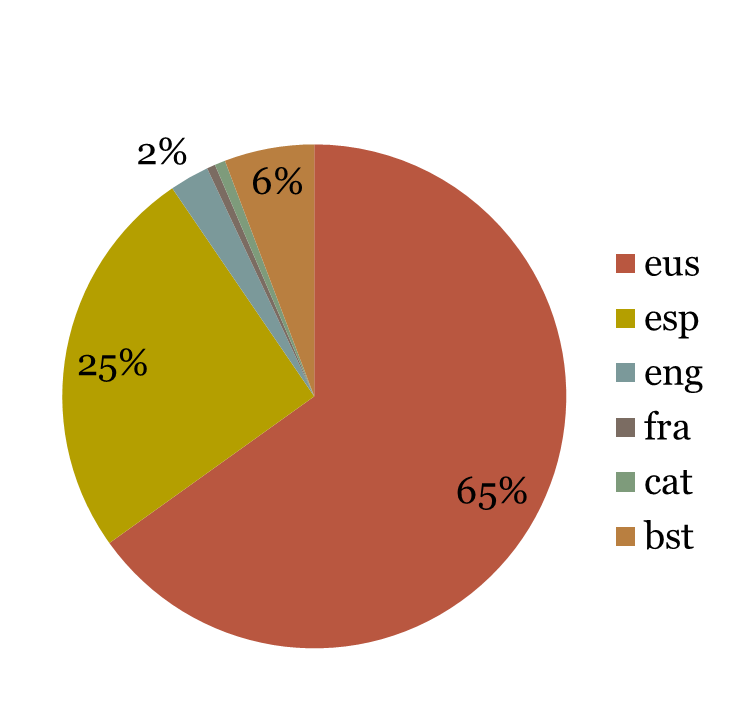
\includegraphics[width=\linewidth]{txio_heldu}
    \caption{Adult personal tweets.}
  \end{subfigure}
  \begin{subfigure}[b]{0.48\linewidth}
    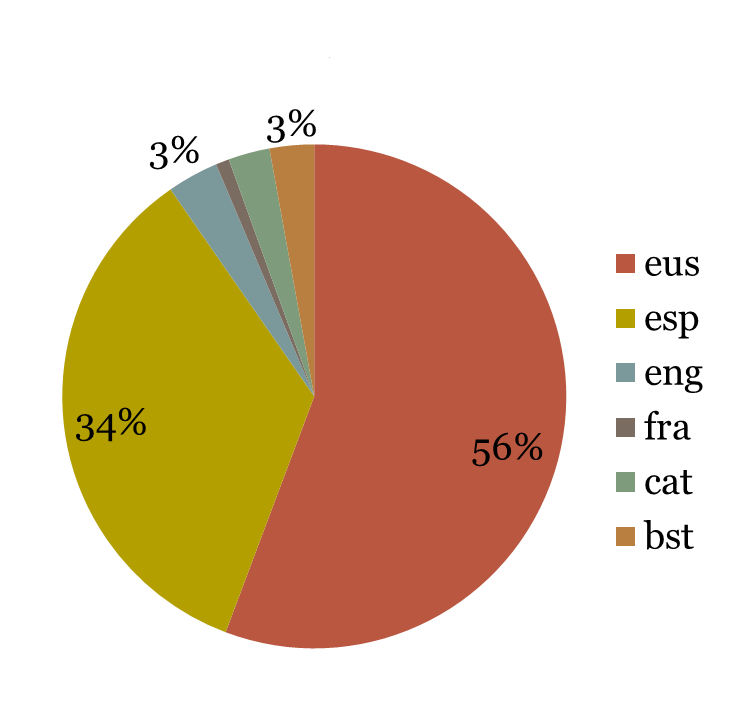
\includegraphics[width=\linewidth]{birtxio_heldu}
    \caption{Adult retweets.}
  \end{subfigure}
  \caption{Adults in the Large Corpus: 5.508 users.}
  \label{fig:adults}
\end{figure}

If we take a look at the tweets written only in Basque, we find that 2.634.534 tweets have been published, containing more than 32M tokens. Figure  \ref{fig:txio luze held} shows their distribution according to their length in tokens. The average tweet contains 12 tokens. Standard deviation with respect to the average is 5.65. Furthermore, median corresponds to 12, mode being 14 token (more than 200K tweets).

\begin{figure}[H]
  \centering
  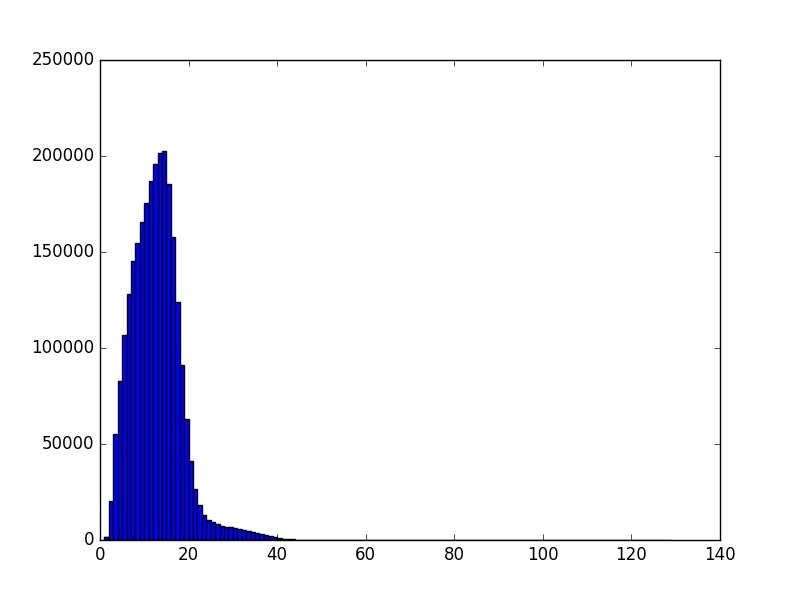
\includegraphics[height=6cm]{graf_for}
  \caption{Distribution of Basque tweets published by adults.}
  \label{fig:txio luze held}
\end{figure}

\subsubsection{Analyzing Young Twitter Users}

The young users corpus contains just one quarter in size with respect to the corpus of adult users. In this case, it can be seen that there are fewer retweets (963.668) than original personal tweets (1.128.124). It is perhaps more noticeable the fact that the use of Basque is less common between young users: 18\% lower for tweets and 24\% lower for retweets. As it is expected, the use of Spanish is higher between young users, reaching 47\% for retweets and 34\% for personal tweets. The data in Figure \ref{fig:gazte txbtx} shows that Basque is less used between young users of Twitter.

\begin{figure}[H]
  \centering
  \begin{subfigure}[b]{0.48\linewidth}
    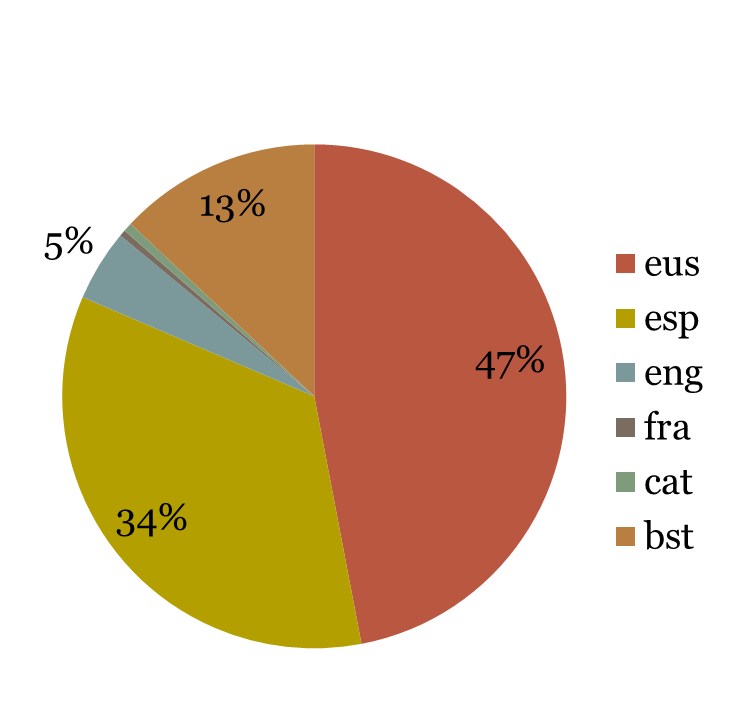
\includegraphics[width=\linewidth]{txio_gazte}
    \caption{Young personal tweets.}
  \end{subfigure}
  \begin{subfigure}[b]{0.48\linewidth}
    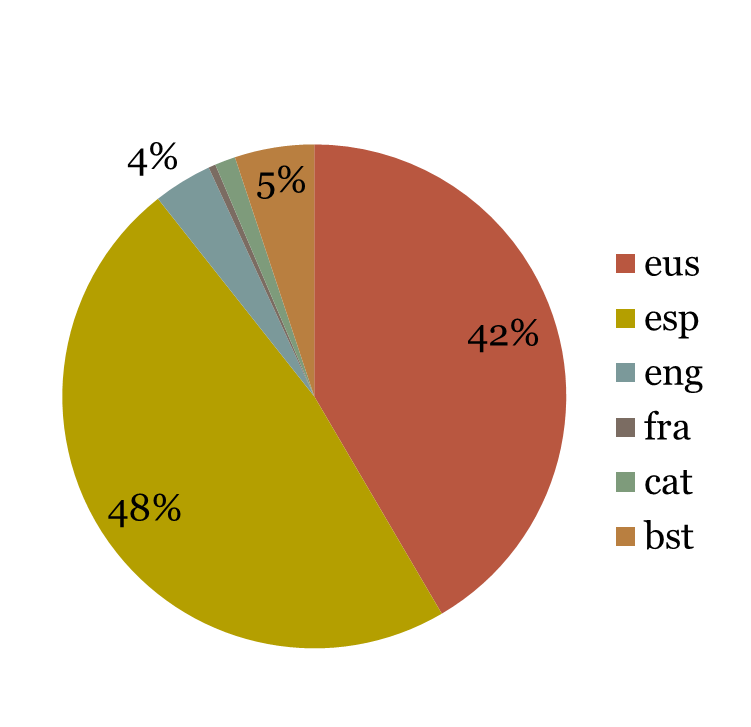
\includegraphics[width=\linewidth]{birtxio_gazte}
    \caption{Young retweets.}
  \end{subfigure}
  \caption{Young users in Large Corpus: 1.579 users.}
  \label{fig:gazte txbtx}
\end{figure}

If we take a look at the tweets written only in Basque, we find that 530.226 personal tweets have been published, containing more than 5M tokens. Figure  \ref{fig:txio luze gzt} shows their distribution according to their length in tokens. The average tweet contains 9 tokens, whereas the standard deviation with respect to the average is 5.49. Furthermore, median corresponds to 8, mode being 6 token (around 45K tweets). In general, it is noticeable the fact that young users published much shorter tweets than adults.

\begin{figure}[H]
  \centering
  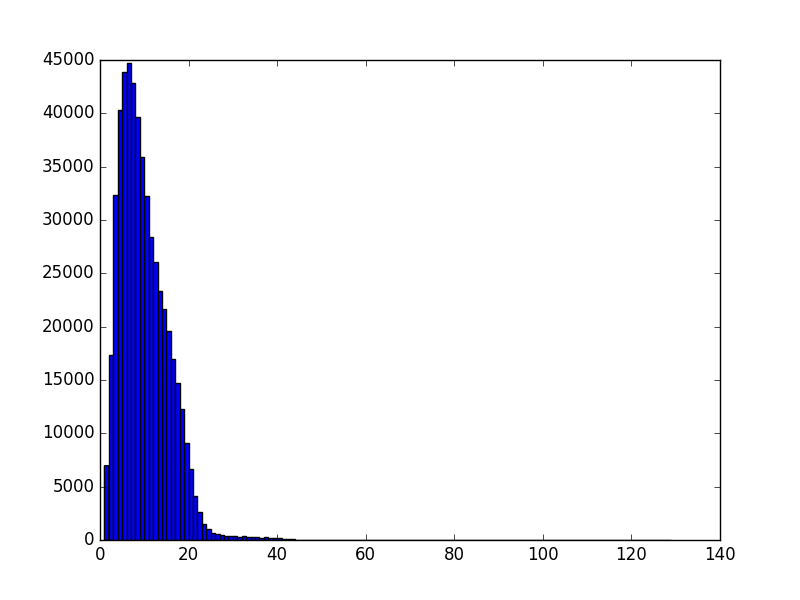
\includegraphics[height=6cm]{graf_inf}
  \caption{Distribution of Basque tweets published by young users.}
  \label{fig:txio luze gzt}
\end{figure}


% ################################################
% ################     TOPICS     ################
% ################################################

\section{Topics}\label{sec:topics}

The aim of this section is to detect the most frequent topics of Twitter users writing in Basque. In order to do so, we start with the personal tweets of users classified as adults and young in the previous section using the classifier developed in Section \ref{sec:ixa}. As shown by Table \ref{tab:largecorpusdata}, more than 3 million personal tweets in Basque were obtained. On the one hand, 2,634,534 personal tweets will be used to predict adult topics and, on the other hand, 530,226 personal tweets for young users. We will apply topic modelling via Latent Dirichlet Allocation (LDA) \cite{blei2003latent} in order to infer relevant topics per type of user from unstructured data. Specifically, we used the implementation of LDA provided by the gensim package \cite{rehurek2010software}.

Topic modeling is a commonly used tool in the field of text mining. With this technique, words are grouped or clustered according to their context, thereby generating more general contents or concepts via the clustered words and allowing to identify general topics from specific words. We apply this technique to identify the main subjects that appear in the Basque users' tweets. In order words, LDA  makes it possible to classify events that are observable in latent or hidden clusters. This is possible thanks to the many hidden features, such as the similarity of words.

Before applying LDA, we need to structured the documents in our dataset. It is difficult to directly apply LDA to our data due to the short length of tweets. Thus, we decide to group the tweets by user, namely, we will create one document per user where the document will be containing every tweet published by that person \cite{hong2010empirical, zhao2011comparing}. Additionally, and considering that Basque is an agglutinative language, we decided to lemmatize the documents to reduce the number of terms that needed to be modelled. For this pre-processing step, the IXA pipes Basque lemmatizer  was used \cite{agerri2014ixa}.

LDA requires to choose a number of topics beforehand. After several tests, 20 topics were used for the adults documents and 12 for the young ones. The different in topics is coherent with the number of tweets for each of user type. Although there is not a fixed correct number of topics, this choice affects the interpretability of the LDA results \cite{binkley2014understanding,steyvers2007probabilistic}. Thus, it is interesting to achieve the most dispersed possible model so that the overlap between topics is kept to a minimum. Furthermore, the resulting topics should correlate with social reality which is latent in the real data.

The results of applying LDA are displayed using LDAvis \cite{sievert2014ldavis}, which allows an easy interpretation of each topic. As it is customary, the identity or meaning of the topic is determined by the words of which it is composed \cite{binkley2014understanding}. Thus, Table \ref{tab:adult-tp} shows the topics obtained for the adult users whereas Table \ref{tab:young-tp} lists the topics for the young users.

\begin{table}[H]
  \centering
  \begin{tabular}{llc}
    \hline
    \textbf{Topics of adult users} &  \textbf{Representative words in the topic} & \textbf{\% of words} \\ \hline \hline
                   1  Conversation & entzun, iruditu, bizitza, pentsatu, pasatu & 10.5  \\
                   & listen, imagine, life, think, pass & \\ \hline
                   2  Politics & Euskal Herri, espainia, politiko, estatu, eskubide & 10.0  \\
                   & Basque Country, Spain, politics, states, rights & \\ \hline
                   3  Basque tweeters & @txargain, @berria, @boligorria, euskara, idatzi & 6.9 \\
                   & @user, @newspaper, @user, Basque, write & \\ \hline
                   4  Cultural offer & lehiaketa, sarrera, ikastaro, erakusketa, antzerki & 6.4  \\
                   & competition, entry, course, exhibition, theater & \\ \hline
                   5  Public administration & udal, zerbitzu, publiko, aurrekontu, euskadi & 6.1  \\
                   & municipal, services, public, budget, euskadi & \\ \hline
                   6  Basque television & @euskaltelebista, urhanditan, @xabiermadariaga, herritxiki & 5.3 \\
                   & @television, TV program, @journalist, TV program & \\ \hline
                   7  Tournaments & txapelketa, final, kirol, jokatu, kanporaketa & 5.0 \\
                   & championship, final, sports, play, playoffs & \\ \hline
                   8  Basque prisoners & preso, herri, espetxe, iheslari, elkartasun & 4.9 \\
                   & prisoner, people, prison, fugitive, solidarity & \\ \hline
                   9  Culture & liburu, literatura, filma, poesia, dokumental & 4.8 \\
                   & books, literature, film, poetry, documentary & \\ \hline
                   10 Social movements & feminista, asanblada, gaztetxe, borroka, langile & 4.8 \\
                   & feminist, assembly, squatted house, fight, worker & \\ \hline
                   11 Education & ikasle, hezkuntza, irakasle, ikastola, ikastetxe & 4.3 \\
                   & students, education, teachers, Basque colleges, schools & \\ \hline
                   12 Science & euskara, artikulu, interesgarri, zientzia, teknologia & 4.1 \\
                   &  Basque, articles, interesting, science, technology& \\ \hline
                   13 Music & kontzertu, disko, talde, entzun, musika & 3.9 \\
                   & concert, disc, group, listen, music & \\ \hline
                   14 Basque language & euskara, hizkuntza, euskaldun, euskal, ikasi & 3.8 \\
                   & Basque language, language, Basque speaker, Basque, learn & \\ \hline
                   15 Sports & talde, real, partida, irabazi, jokatu & 3.8 \\
                   & team, real, match, win, play & \\ \hline
                   16 Gipuzkoa & tolosa, andoain, hernani, ordizi, beasain & 3.7  \\ \hline
                   17 Media in Basque & @berria, @euskalirratia, @argia, @zebrabidea, @iehkohitza & 3.5  \\ \hline
                   18 Donostia & donostia, @donostiakoudala, ezagutu, gipuzkoa & 3.5  \\ \hline
                   19 Nafarroa & nafarroa, baztan, altsasu, irunerri, irun & 2.7  \\ \hline
                   20 Bizkaia & larrabetzu, lekeitio, durango, bermeo, arrasate & 2.6 \\ \hline
  \end{tabular}
  \caption{Topics of adult users. Whenever necessary, English translation is provided below each row of representative words.}
  \label{tab:adult-tp}
\end{table}


\begin{table}[H]
  \centering
  \begin{tabular}{llc}
    \hline
    \textbf{Topics of young users} &  \textbf{Representative words in the topic} & \textbf{\% of words} \\ \hline \hline
                   1  Gipuzkera dialect (informal chat) & in, ne, oain, atxalde, biyar & 14.7 \\
                   & do, mine, now, late, tomorrow & \\ \hline
                   2  Express feelings & maite, amets, gau, bizi, bihotz & 11.4 \\
                   & love, dream, night, live, heart & \\ \hline
                   3  Bizkaiera dialect (informal chat) & dau, be, ein, dot, emun, bixar & 10.8 \\
                   & is, also, do, have, give, tomorrow & \\ \hline
                   4  Sports & partidu, irabazi, jokatu, txapeldun, etapa & 9.9 \\
                   & match, win, play, champion, stage & \\ \hline
                   5  Cultural activities & areto, antzoki, gaztetxe, tailer, kontzertu & 9.7 \\
                   & halls, theaters, youth clubs, workshops, concerts & \\ \hline
                   6  To congratulate & zorion, pasatu, animo, eskerrikasko, polit & 9.3 \\
                   & congratulations, pass, courage, thank you, nice & \\ \hline
                   7  Tell the life & jajaja, bihar, ohera, partido, ikasi & 7.6 \\
                   & Hahaha, morning, to bed, party, study & \\ \hline
                   8  Bizkaiera dialect (formal chat) & dot, dau, barri, barik, be & 7.1 \\
                   & have, is, new, without, too & \\ \hline
                   9  Gipuzkera dialect (formal chat) & det, ne, hoi, iruditu, irakurri  & 7.1 \\
                   & do, mine, that, seem, read & \\ \hline
                   10 Basque prisoners & herri, euskal, etxe, preso, gazte & 6.4 \\
                   & people, Basque, house, prisoner, youth & \\ \hline
                   11 Athletic CB & aupa, athletic, @athletic, san mames, bilbo  & 3.3 \\ \hline
                   12 Rowing & sailkapen, jardunaldi, maila, txapelketa, estropada & 2.7 \\
                   & classification, event, level, championship, regatta & \\ \hline
  \end{tabular}
  \caption{Topics of young users. Whenever necessary, English translation is provided below each row of representative words.}
  \label{tab:young-tp}
\end{table}

The topics from adult users show that they mostly talk about politics, social, cultural and linguistic (Basque language-related) issues. It is also interesting to notice that public institutions also appear in the social network, such as Basque Country regional offices from Gipuzkoa, Bizkaia or Nafarroa. However, if we look at the topics most common between young users (Table \ref{tab:young-tp}) we can see that they are mostly related to everyday affairs (chatting between friends, expressing feelings and emotions with respect to something, etc.). In some cases, they talk about everyday issues using their local Basque dialect (e.g., \emph{Gipuzkera} and \emph{Bizkaiera}). Additionaly, sports (Athletic Club, rowing) are also a recurring theme among young people. Thus, comparing the two different age stages, it should be noted that young people use Twitter for more day-to-day activities among friends or among contacts within the network. In the case of adults, it is clear that there is more political and social content.


% ################################################
% ################    RELATIONS   ################
% ################################################

\section{Relations}\label{sec:connections}

In this section we will study the relations that appear between Basque users of Twitter. As in the previous section, the starting point will be the retweets of users classified as \emph{adult} or \emph{young} using the classifier developed in Section \ref{sec:ixa}. The number of retweets for each type of users are reported in Table \ref{tab:largecorpusdata}. Specifically, 2,421,058 retweets will be used to study the relations that are created between adult users. With respect to young users, the corpus consists of 400,448 retweets. The overall objective is to uncover the most important relations formed between users by studying the links between their retweets and comparing the different behaviour and relations of young and adult users.

First, we created a giant graph using the data (retweets) for each type of user. To build the graph, two features extracted from each retweet were used: (i) who retweets and (ii) who has been retweeted. Thus, the data source will be the source and the target of each retweet. Based on these two characteristics, the two graphs were created using the \textit{gephi} program \cite{bastian2009gephi}.

Once the graphs were created, we proceed as follows: First, we divided each graph into subgroups using the modularity algorithm \cite{blondel2008fast}. Second, we gave the network a spatial structure by using the \textit{ForceAtlas2} algorithm \cite{jacomy2014forceatlas2}, ordering the nodes according to the community to which they belong. Finally, the identity of each subgroup or community was defined, using the most important nodes of the created subgroups. By doing so it can be seen how the communities within each graph are structured.

Thus, in the adult graph we identified 33,277 nodes whereas 24,987 nodes were identified among the young users. Once the two independent network graphs, one for young users and another one for adults, were created, we split each network into subgroups to analyze how the communities or subgroups inside each one are formed. The subgroups are defined based on their most important nodes. The aim is to uncover, via their retweets, the relations that are created between the Basque users of Twitter. As an example of the graphs obtained, Figure \ref{fig:hd ha2} displays the two most important subgroups within the adult and young graphs, respectively.

\begin{figure}[H]
  \centering
  \begin{subfigure}[b]{0.49\linewidth}
    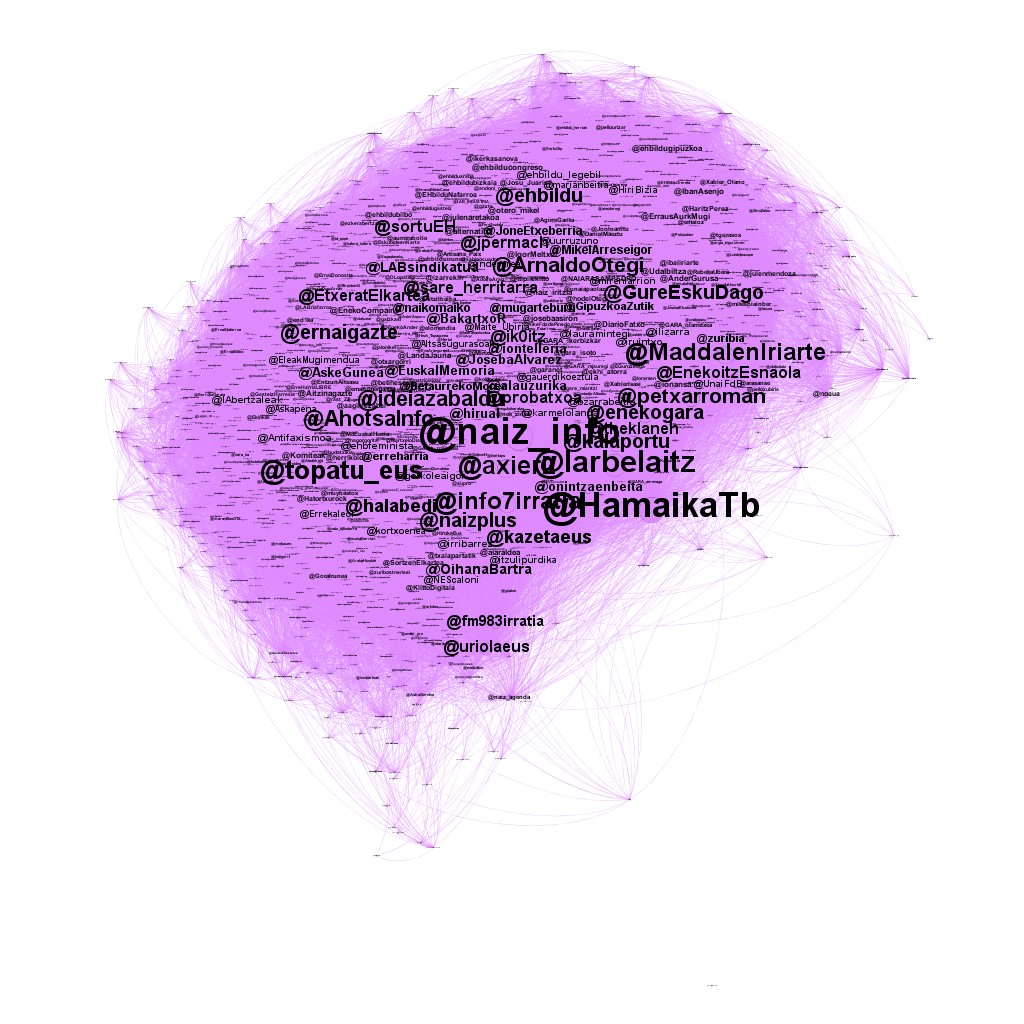
\includegraphics[width=\linewidth]{adult_graphs/c1for}
    \caption{Most important community (Nationalist left) in the adult graph.}
  \end{subfigure}
  \begin{subfigure}[b]{0.49\linewidth}
    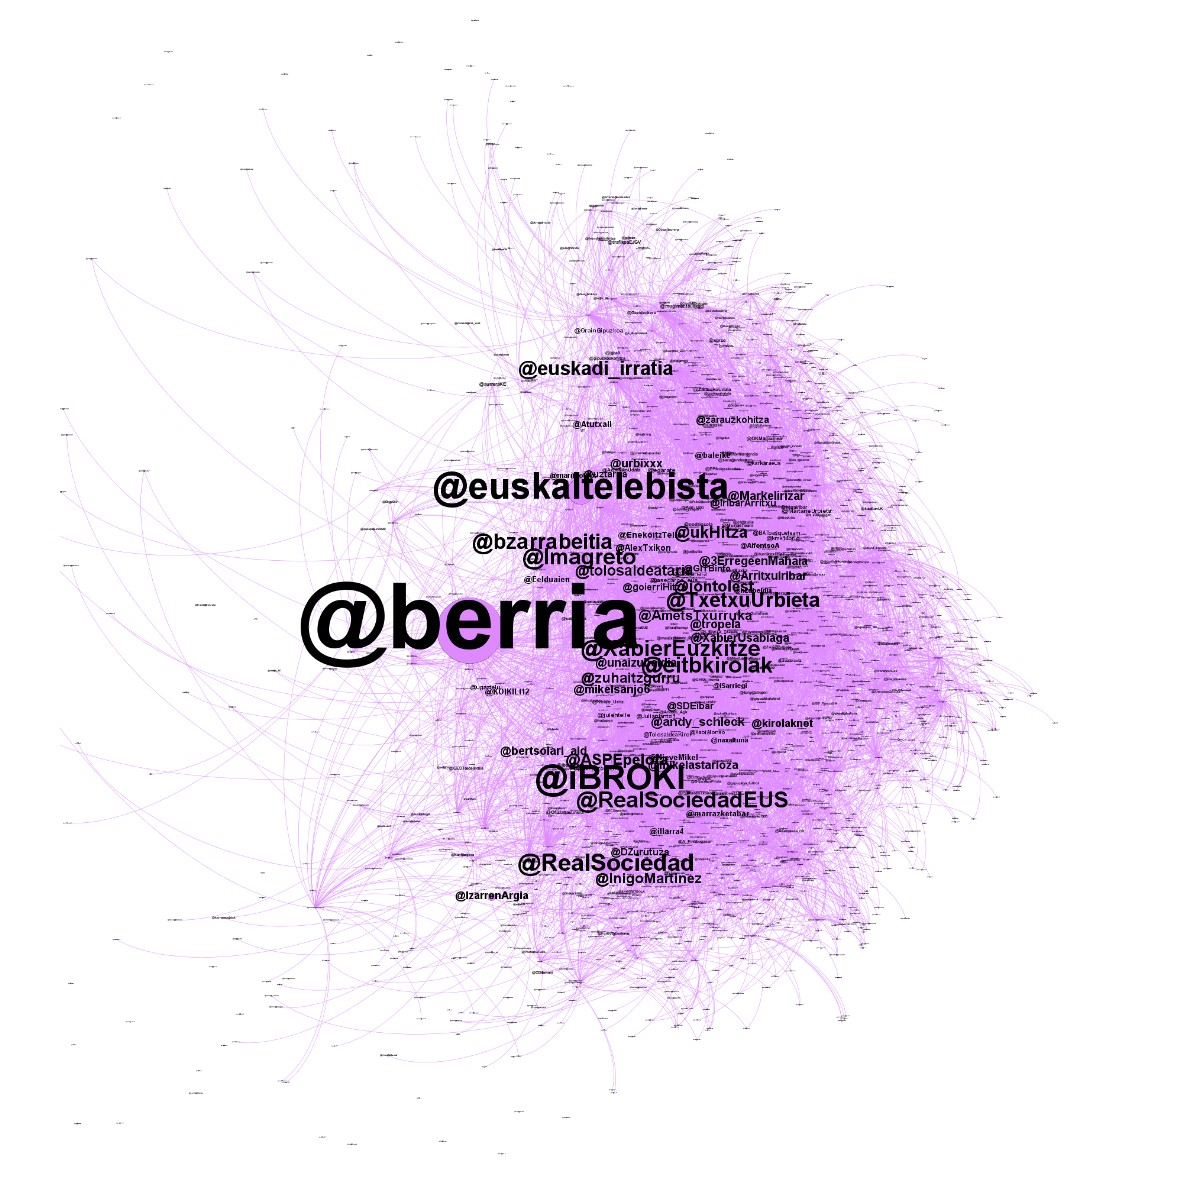
\includegraphics[width=\linewidth]{young_graphs/c1inf}
    \caption{Most important community (Sports) in the young graph.}
  \end{subfigure}
  \caption{Example graphs of the two most important subgroups within the adult and young graphs.}
  \label{fig:hd ha2}
\end{figure}

\subsection{Relationships in the Adult Graph}\label{sec:sis harr}

\begin{table}[H]
  \centering
  \begin{tabular}{lllll} \hline
    Nationalist left  &  News & Basque language & Music and GED & Basque users \\ \hline \hline
    @naiz\_info &  @berria &  @zuzeu &  @XMadariagaI &  @boligorria \\
    @HamaikaTb &  @eitbAlbisteak &  @KikeAmonarriz &  @gaizkapenafiel &  @zaldieroa \\
    @larbelaitz & @euskaltelebista &  @Sustatu &  @JGGarai &  @urtziurkizu \\
    @topatu\_eus &  @euskadi\_irratia &  @Gaztezulo &  @EsneBeltza & @landergarro \\
    @axierL & @tolosaldeataria & @AEK\_eus  & @UrHanditan  &  @ielortza\\ \hline
  \end{tabular}
  \caption{Most important nodes for the subgroups in the graph of adult users.}
  \label{tab:tab harr hld}
\end{table}

Table \ref{tab:tab harr hld} shows the five main subgroups derived from the graph of \textbf{adult} users. Each of the subgroups displays a common characteristic, namely, that all of them have a direct relation with topics or issues related to the Basque Country. Thus, it can be seen that for adult users Basque language is used to talk mostly about Basque issues, highlighting politics (Separatist left) and current affairs (news). In other words, the main function is to talk about politics and social issues but with a clear focus on the Basque community itself (rather than on international affairs). In the following we describe the main characteristics of each of the subgroups contained in the graph of adult users.

\begin{itemize}

\item \textbf{Nationalist Left} (27.92\%): This subgroup is made up of nodes with a specific political orientation, mostly related to members of the Nationalist Left. In addition to the users that appear in the first column of Table \ref{tab:tab harr hld}, there are also many important nodes that refer to specific users (@ArnaldoOtegi, @jpermach, @JosebaAlvarez...) or institutions (@sortuEH, @LAB...) of the Nationalist Left. This is the main group, joined by more than a quarter of all nodes that corresponds to the relationship of a certain political orientation.

\item \textbf{News} (23.77\%): This group, related to news, consists of almost a quarter of all users. Most of the nodes of this subgroup are related to the media, specially several users related to the Basque public television (EITB).

\item \textbf{Basque language} (15.34\%): In the 3rd subgroup, there are topics related to the Basque language, such as communication media in Basque (@zuzeu, @Gaztezulo, @ArabakoALEA), associations for the promotion of the Basque language (@AEK\_eus, @EHEbizi...) as well as several individuals related to the Basque language (@KikeAmonarriz, @KoldoTellitu, @MertxeMugika).

\item \textbf{Music and GED} (13.56\%): In the fourth subgroup there is a special phenomenon, since it brings together two different groups in the same subgroup. The first one is related to music, since we can appreciate different users related to the music scene (@EsneBeltza, @ZuriHidalgo, @ZeEsatek, @40minuturock, @hesiantaldea, @ItzrrSemeak ...). The second one is related to the users of the social movement ``Gure Esku Dago'' (@GoierrikoGED, @GEDTolosaldea, @GureEskuDagoDon ...).

\item \textbf{Basque tweeters} (13.10\%): In this last subgroup we can find popular Basque users of Twitter, which are important within the Basque community due to their large number of followers or retweets.
\end{itemize}

\subsection{Relationships in the Young Graph}\label{sec:relat-young-subgr}

The subgroups in the graph of \textbf{young} users (see Table \ref{tab:tab harr gzt}) display both similarities and differences with respect to the adult graph.

\begin{table}[H]
  \centering
  \begin{tabular}{lllll} \hline
    Sports & Basque language & Nationalist left & News & Music \\ \hline \hline
     @berria &  @enekogara & @naiz\_info & @argia & @berritxarrak \\
     @euskaltelebista & @GureEskuDago & @larbelaitz &  @HamaikaTb & @gaztea \\
     @iBROKI & @EsaldiakEuskara & @topatu\_eus &  @eitbAlbisteak & @izanpirata \\
     @RealSociedad & @ZuriHidalgo & @ArnaldoOtegi & @MaddalenIriarte & @eitbeus \\
     @XabierEuzkitze & @MeriLing1 & @ernaigazte & @ielortza & @LeakoHitza \\ \hline
  \end{tabular}
  \caption{Most important nodes for the subgroups in the graph of young users.}
  \label{tab:tab harr gzt}
\end{table}

Focusing on the similarities, \textit{Basque language}, \textit{Nationalist left} and \textit{News} are important subgroups in both graphs. These common subgroups can be related to politics and immediacy, which are basic characteristics of identity in Twitter. With respect to the differences, it noticeable that subgroups related to leisure take a more central stage, such as \textit {Sports} and \textit{Music}. Moreover, it is worth pointing out that young Basque users take Twitter as a channel to comment on everyday issues. Finally, the main topics in each of the subgroups within the young users graphs are listed in the following:

\begin{itemize}
\item \textbf{Sports} (21.61\%): This subgroup, which includes most of the nodes which are considered roles models for the youths, is related to sports. The group is be made up of sports teams or organizations (@RealSociety, @RealSociedadEUS, @ASPEpelota, @SDEibar ...), as well as its athletes (@InigoMartinez, @AmetsTxurruka, @XabierUsabiaga, @Markelirizar ...). However, the most important nodes are sports journalists (@iBROKI, @XabierEuzkitze, @Imagreto, @bzarrabeitia, @TxetxuUbieta...) and the media (@berria, @euskaltelebista, @eitbkirolak, @euskadi\_irratia...). Once again, it can be clearly seen that the newspapers and TV media are the most important nodes.

\item \textbf{Basque language} (20.70\%): A fifth of all the nodes are in this subgroup. The most important ones are those directly related to the Basque language (@EsaldiakEuskara, @euskarazEH, @Bertsotan, @bertsolaritza, @Euskeraz\_Bizi ...). In the adult graph it was also found a community related to this topic, although the most important nodes are markedly different.

\item \textbf{Nationalist left} (17.12\%): This third group, composed of nodes related to the nationalist left, is perhaps the most similar in both adult and young graphs. For example, media (@naiz\_info, @topatu\_eus, @inform7irratia, @naizplus...), organizations (@ernaigazte, @ehbildu, @sortuEH...) and individuals (@ArnaldoOtegi, @lauramintegi...) related to the nationalist left, appear in both subgroups.

\item \textbf{News} (14.92\%): As in the previous subgroup, this community is also very similar for both young and adult users. The most important nodes correspond to general news Basque media (@argia, @HamaikaTb, @eitb Albums, @zuzeu, @Gaztezulo).

\item \textbf{Music} (11.35\%): In this final subgroup, although quite heterogeneous, it can be said that the most important nodes are related to music. Among these, the music related media (@gaztea, @DidaGaztea), music bands (@berritxarrak, @muguruzafm, @Glaukomaband), as well as record companies (@BagaBigaeus) are the main nodes.

\end{itemize}

To finish this section, Table \ref{tab:taldeak} offers an overview of the main subgroups per type of user. Both graphs create communities related to political and social issues, although it is more important for the graph of young users. Moreover, in both types of users Basque language is an important subgroup and it shows that users write in Basque mostly about issues or topics directly related to the Basque Country. The main difference between both types of users is the importance of the sports subgroup which is not present in the graph of adult users. This shows the influence of sports celebrities as role models among young people.

\begin{table}[H]
           \centering
           \captionsetup[subtable]{position = below}
          \captionsetup[table]{position=top}
           \begin{subtable}{0.45\linewidth}
               \centering
               \begin{tabular}{lc}\hline
                   Subgroups in graph of adult users & \% of nodes \\ \hline \hline
                   Nationalist left & 27.92 \\
                   News & 23.77 \\
                   Basque language & 15.34 \\
                   Music and GED & 13.56 \\
                   Basque tweeters & 13.10 \\ \hline
               \end{tabular}
           \end{subtable}%
           \hspace*{4em}
           \begin{subtable}{0.45\linewidth}
               \centering
               \begin{tabular}{lc}\hline
                   Subgroups in graph of young users & \% of nodes \\ \hline \hline
                   Sports & 21.61 \\
                   Basque language & 20.70 \\
                   Nationalist left & 17.12 \\
                   News & 14.92 \\
                   Music & 11.35 \\ \hline
               \end{tabular}
           \end{subtable}
           \caption{Communities in each graph of users.}
           \label{tab:taldeak}
       \end{table}


% ####################################################
% ################     CONCLUSION     ################
% ####################################################

\section{Conclusion and Future Work}\label{sec:conclusion}

We have shown how to develop different systems that allows us an approximation to the reality of certain communities of Twitter, in this case to the community of Basque speakers. The first step has allowed the collection of large amounts of information based on the target community. The second step has allowed the segmentation of the extracted sample by life stage, demonstrating that it is possible to segment by demographic features. In third and last place, we can show the topics of conversation and the relationships of young and adults, showing the reality of two different groups. In general terms, it is proven that the social sciences and computer science make a good combination thanks to the application of language processing techniques,, demonstrating that demographic features can be inferred and that social interactions can be discovered.

It can be said that a new data source has been opened thanks to the possibility of extracting information from Twitter. This extraction technique has allowed to achieve large amounts of data at a very low cost. It would be interesting to extend the extraction of data to other social networks such as Instagram and Facebook, which due to their closure make it very difficult to extract their data. However, this new source of data also has its limits in research, since it leaves out, at least for now, a part of the population. Even so, it must be admitted that a successful system has been developed, getting more than 10 million tweets in Basque from almost 8,000 different users, a considerable amount of data dealing with a minority language. An important part of this research is based on the segmentation between young people and adults, since the prediction of demographic characteristics is an important tool for social research. The distinction between youth and adults is not based on age, it has been done according to the formality of the text, since age-based labeling was too expensive. Therefore, given the difficulties of age labeling, it is decided to use a methodological shortcut, if the concentration of informal text is high, the author will be considered as young. For the future, it would be appropriate to carry out the classification by age, investing more resources but making a more real approach. Thanks to the document classifier of IXA pipes, good results have been achieved, demonstrating that it is a robust system that works well with small training corpus, making it possible for small researchers to do their job well.

Once the entire sample has been segmented between young people and adults, it has been possible to show the topics of which they speak and how do they interact. First of all, what Basque users speak about has been shown. Most young people use this social network to communicate with nearby people about everyday events. On the other hand, among adults it would function more as an instrument of expression, especially when it comes to publishing topics that are political or current in nature. Despite the different themes of adults and young people, this social network is used mainly as a means of communication and information exchange. Second, we have been able to identify the different subgroups within the same community, using the interactions or retweets. In addition, it is worth mentioning that users related to the media play an important role, confirming the informative nature of Twitter. Basque users use Basque, especially to talk about events or topics related to them. It can be said that the communities are easily identifiable and can be related to the context of the Basque Country, showing that the approach is useful. It can be concluded by saying that Basque is used mainly to talk about the subjects of the Basque people.

Thanks to this work, it has been possible to discover how Basque language is adapting to the context of the 21st century, demonstrating that it is present in social networks, with more than 6 million tweets in Basque and almost 8,000 different users crawled. Being present in new technologies, such as social networks, means that our language is able to adapt to new challenges, thanks to the creativity of the Basques to introduce them into these spaces. As the result of this research, it can be said that Basque speakers use Basque language to speak about their own issues, showing that Basque language is capable of adapting to new contexts, always being linked to the everyday reality of the community of speakers. This shows, in this globalized and constantly connected world, that the Basques have a special ability to find their place and settle down.

%%%%%%%%%%%%%%%%%%%%%%%%%%%%%%%%%%%%%%%%%%
\vspace{6pt}

%%%%%%%%%%%%%%%%%%%%%%%%%%%%%%%%%%%%%%%%%%
%% optional
%\supplementary{The following are available online at \linksupplementary{s1}, Figure S1: title, Table S1: title, Video S1: title.}

% Only for the journal Methods and Protocols:
% If you wish to submit a video article, please do so with any other supplementary material.
% \supplementary{The following are available at \linksupplementary{s1}, Figure S1: title, Table S1: title, Video S1: title. A supporting video article is available at doi: link.}

%%%%%%%%%%%%%%%%%%%%%%%%%%%%%%%%%%%%%%%%%%
\authorcontributions{Conceptualization, JFdL, RA and IA; methodology, JFdL, RA and IA; software, JFdL, RA and IA; formal analysis, JFdL, RA, IA; data curation, JFdL and RA; writing—original draft preparation, RA and JFdL; writing—review and editing, RA; supervision, RA and IA.}

%%%%%%%%%%%%%%%%%%%%%%%%%%%%%%%%%%%%%%%%%%
\funding{The second author is funded by the Spanish Ministry of Economy and Competitiveness (MINECO/FEDER, UE), under the project CROSSTEXT (TIN2015-72646-EXP) and the Ramon y Cajal Fellowship RYC-2017-23647. He also acknowledges the support of the BBVA Big Data 2018 ``BigKnowledge for Text Mining (BigKnowledge)'' project.}

%%%%%%%%%%%%%%%%%%%%%%%%%%%%%%%%%%%%%%%%%%
\acknowledgments{We gratefully acknowledge the support of NVIDIA Corporation with the donation of the Titan V GPU used for this research.}

%%%%%%%%%%%%%%%%%%%%%%%%%%%%%%%%%%%%%%%%%%
%\conflictsofinterest{Declare conflicts of interest or state ``The authors declare no conflict of interest.'' Authors must identify and declare any personal circumstances or interest that may be perceived as inappropriately influencing the representation or interpretation of reported research results. Any role of the funders in the design of the study; in the collection, analyses or interpretation of data; in the writing of the manuscript, or in the decision to publish the results must be declared in this section. If there is no role, please state ``The funders had no role in the design of the study; in the collection, analyses, or interpretation of data; in the writing of the manuscript, or in the decision to publish the results''.}

%%%%%%%%%%%%%%%%%%%%%%%%%%%%%%%%%%%%%%%%%%
%% optional
%\abbreviations{The following abbreviations are used in this manuscript:\\

%\noindent
%\begin{tabular}{@{}ll}
%MDPI & Multidisciplinary Digital Publishing Institute\\
%DOAJ & Directory of open access journals\\
%TLA & Three letter acronym\\
%LD & linear dichroism
%\end{tabular}}

%%%%%%%%%%%%%%%%%%%%%%%%%%%%%%%%%%%%%%%%%%
%% optional
% \appendixtitles{no} %Leave argument "no" if all appendix headings stay EMPTY (then no dot is printed after "Appendix A"). If the appendix sections contain a heading then change the argument to "yes".
% \appendixsections{multiple} %Leave argument "multiple" if there are multiple sections. Then a counter is printed ("Appendix A"). If there is only one appendix section then change the argument to "one" and no counter is printed ("Appendix").
% \appendix
% \section{}
% \unskip
% \subsection{}
% The appendix is an optional section that can contain details and data supplemental to the main text. For example, explanations of experimental details that would disrupt the flow of the main text, but nonetheless remain crucial to understanding and reproducing the research shown; figures of replicates for experiments of which representative data is shown in the main text can be added here if brief, or as Supplementary data. Mathematical proofs of results not central to the paper can be added as an appendix.

% \section{}
% All appendix sections must be cited in the main text. In the appendixes, Figures, Tables, etc. should be labeled starting with `A', e.g., Figure A1, Figure A2, etc. 

%%%%%%%%%%%%%%%%%%%%%%%%%%%%%%%%%%%%%%%%%%
% Citations and References in Supplementary files are permitted provided that they also appear in the reference list here. 

%=====================================
% References, variant A: internal bibliography
%=====================================
\reftitle{References}
\externalbibliography{yes}
\bibliography{biblio,references}


%\begin{thebibliography}{999}
%% Reference 1
%\bibitem[Author1(year)]{ref-journal}
%Author1, T. The title of the cited article. {\em Journal Abbreviation} {\bf 2008}, {\em 10}, 142-149, doi:xxxxx.
%% Reference 2
%\bibitem[Author2(year)]{ref-book}
%Author2, L. The title of the cited contribution. In {\em The Book Title}; Editor1, F., Editor2, A., Eds.; Publishing House: %City, Country, 2007; pp. 32-58, ISBN.
%\end{thebibliography}

%=====================================
% References, variant B: external bibliography
%=====================================
%\externalbibliography{yes}
%\bibliography{your_external_BibTeX_file}

%%%%%%%%%%%%%%%%%%%%%%%%%%%%%%%%%%%%%%%%%%
%% optional
%\sampleavailability{Samples of the compounds ...... are available from the authors.}

%% for journal Sci
%\reviewreports{\\
%Reviewer 1 comments and authors’ response\\
%Reviewer 2 comments and authors’ response\\
%Reviewer 3 comments and authors’ response
%}

%%%%%%%%%%%%%%%%%%%%%%%%%%%%%%%%%%%%%%%%%%
\end{document}
